\documentclass[11pt]{article}

\usepackage[T1]{fontenc}
\usepackage{lmodern}
\usepackage[margin=1in]{geometry}
\usepackage{microtype}
\usepackage{amsmath,amssymb}
\usepackage{booktabs}
\usepackage{graphicx}
\usepackage{xcolor}
\usepackage[round,authoryear]{natbib}
\usepackage{caption}
\usepackage{subcaption}
\usepackage{enumitem}
\usepackage{multirow}
\usepackage{float}
\usepackage{tikz}
\usetikzlibrary{arrows.meta,positioning,fit,calc,shapes.geometric}
\usepackage[hidelinks]{hyperref}

\definecolor{gcol}{HTML}{0072B2}
\definecolor{hcol}{HTML}{D55E00}
\definecolor{elocol}{HTML}{7F7F7F}
\definecolor{boxfill}{HTML}{F2F5F9}

\captionsetup{font=small,labelfont=bf}
\setlist{itemsep=2pt,topsep=4pt}
\graphicspath{{figures/}}

\newcommand{\neurhl}{NeurHL}
\newcommand{\neurhlH}{NeurHL-H}
\newcommand{\neurhlG}{NeurHL-G}
\newcommand{\ci}[2]{[$#1$, $#2$]}

\title{\textbf{NeurHL: A Preregistered Study of Neural Forecasting\\in the National Hockey League}}
\author{ph05\\[2pt]\small\url{https://github.com/ph05/neurhl}}
\date{September 2026}

\begin{document}
\maketitle

\begin{abstract}
\noindent
Forecasting single NHL games is a problem of small margins. The log-loss gap
between a constant home-win rate and a well-tuned rating system is about 0.02
nats, and genuine improvements on such a system are measured in thousandths.
Improvements of that size are easily manufactured by evaluating on data that
shaped the model. We describe \neurhl{}, a forecasting system for NHL games,
skaters and seasons developed under a preregistration protocol: evaluation
windows fixed by season before modelling, data loaders that refuse sealed
seasons, causality audits, capped search ledgers, and one-shot confirmatory
tests committed before their data were scored. Two results were confirmed. A
neural player-level model aggregated over each game's dressed lineup and
combined with Elo in a thin logistic head (\neurhlH{}) beat a tuned Elo system on
10,184 held-out games from 2017--18 to 2025--26: log loss 0.66495 against
0.66973, a difference of $-0.00478$ (95\% CI $-0.00650$ to $-0.00306$), better in
all eight seasons, with the gain coming from resolution rather than
calibration. A chained gradient-boosted model of ice time, shots, goals and
assists beat each skater's own recent average on all four targets over 130,092
held-out skater-games. A third model, \neurhlG{}, simulates a full box score for
each game from the two lineups under exact ice-time conservation and a
score-and-time hazard. On its gate seasons it beat Elo by 0.0056 but was level
with \neurhlH{}, so its preregistered pre-gate failed and its sealed test was not
spent. We report the null results in full: neural event embeddings that encode
a player's type but not his team's strength, two information leaks that passed
every realism gate, a drift in how shot locations are recorded, and an error in
our own gate implementation found while writing this paper. Every 2026--27
forecast is committed before its game and will be scored once, at the end of
the season.
\end{abstract}

\section{Introduction}
\label{sec:intro}

Ice hockey is among the least predictable of the major professional sports.
Goals are rare, around three per team per game, and a single deflection can
decide a result, so even a large difference in team quality translates into a
modest difference in win probability \citep{bennaim2006parity,lopez2018often}. For the
National Hockey League (NHL) the consequence is a narrow band of achievable
skill. On our tuning seasons a constant home-win rate scores a log loss of
0.6887 per game and a tuned Elo system \citep{elo1978rating,hvattum2010using}
scores 0.6759. Betting markets, the usual reference for the best achievable
forecast \citep{strumbelj2014determining}, are better still; our plans worked
with a rough closing-line figure of 0.66, which we could not verify because
the project uses no market data. The competition between forecasting methods
therefore takes place inside a few hundredths of a nat, and a genuine
improvement over a good rating system is a few thousandths.

Effects that small are fragile. Repeatedly trying configurations against the
same held-out seasons will eventually produce one that looks better by chance
\citep{simmons2011false,gelman2014statistical}, and information that leaks from
the future into features produces gains that vanish in use
\citep{kaufman2012leakage,kapoor2023leakage}. A model with no skill at all
would clear a 0.002-nat improvement bar on our tuning window by chance about
23\% of the time (Section~\ref{sec:protocol}). Preregistration, the practice of
committing hypotheses, analyses and decision rules before the data that test
them exist, is now standard in parts of the experimental sciences
\citep{nosek2018preregistration}, and templates for preregistering predictive
models have been proposed \citep{hofman2023preregistration}, but it remains
rare in the predictive modelling of sport.

This paper reports \neurhl{}, a system that forecasts NHL games, skaters and
seasons, built across four successive preregistrations. Each plan was committed
to the project's repository before any number that tested it was computed, and
the repository, with its full history, is public. Seasons
were assigned to development, tuning, confirmation and live roles before any
model was fitted, and the code refuses to score across those boundaries. Every
configuration searched was logged against a declared cap. Each confirmatory
test was run once, after a freeze commit, by a script that refuses a second
run. The record of what failed is kept as carefully as the record of what
worked.

Our contributions are:
\begin{enumerate}
  \item \textbf{A preregistration protocol for sports forecasting} with season
  windows, guarded data loaders, causality audits that corrupt the future and
  require the past to be bit-identical, capped search ledgers, one-shot tests,
  and a live scoring rule under which a forecast counts only if it is publicly
  committed before its game starts (Section~\ref{sec:protocol}).
  \item \textbf{A confirmed game-level improvement over Elo.} \neurhlH{} conditions
  on the dressed lineup through a neural player-level model and combines the
  result with Elo in a four-feature logistic head. On 10,184 held-out games it
  improves log loss by 0.00478 (95\% CI 0.00306 to 0.00650), in all eight
  seasons, and increases Elo's skill over the home-win base rate by about a
  quarter (Section~\ref{sec:res-h}).
  \item \textbf{A confirmed player-game model} of ice time, shots, goals and
  assists that beats each skater's own recent average on all four targets
  (Section~\ref{sec:res-pg}).
  \item \textbf{\neurhlG{}, a single-game simulation engine} that produces a full
  box score from the two lineups. Ice time is conserved exactly by
  construction, player outputs sum to team totals, and the outcome comes from a
  differentiable integration of a score-and-time hazard over the goal
  differential. It beats Elo on its gate seasons but adds no demonstrable
  win-probability information beyond \neurhlH{}, so its sealed test was not spent
  (Section~\ref{sec:res-g}).
  \item \textbf{A record of null results and failure modes}
  (Sections~\ref{sec:res-nulls} and~\ref{sec:failures}): pooled neural event
  embeddings that carry no team-strength signal; tree ensembles and wide
  networks that do not beat Elo; two leaks that passed every realism gate; a
  recording drift that changed what a shot location means; and implementation
  errors in our own gates, one of them found while writing this paper.
\end{enumerate}

Section~\ref{sec:related} places the work in context, Section~\ref{sec:data}
describes the data, Section~\ref{sec:protocol} the protocol and
Section~\ref{sec:models} the models. Section~\ref{sec:results} reports results,
Section~\ref{sec:failures} the failures and corrections,
Section~\ref{sec:live} the prospective test running during the 2026--27
season, and Section~\ref{sec:discussion} what we take from all of it. We name
seasons by the year in which they end, so 2018 is the 2017--18 season.

\section{Related work}
\label{sec:related}

\paragraph{Rating systems and game forecasting.}
Elo's rating system \citep{elo1978rating} updates a scalar strength after
each result in proportion to the surprise. In association football it has been
shown to be a strong basis for match forecasts \citep{hvattum2010using}, and
variants with margin-of-victory multipliers and between-season regression are
widely used for the NHL; \citet{whelan2021bradley} generalise the related
Bradley--Terry model to hockey's regulation, overtime and shootout outcomes.
Goal-based models descend from the independent Poisson model of
\citet{maher1982modelling} and its dependence correction by
\citet{dixon1997modelling}, and \citet{kaplan2014markov} derive in-game win
probabilities from a Markov model of goal and manpower differentials. For NHL
games, \citet{weissbock2013use} classified winners from traditional and
possession statistics and reached about 59\% accuracy, well below what similar
methods achieve in other sports, and \citet{gu2019game} combined player and
team data in ensemble learners. Both findings fit analyses that place hockey
among the most random of the major sports
\citep{bennaim2006parity,lopez2018often}. Betting markets are the usual
reference for the best achievable forecast
\citep{strumbelj2014determining,wunderlich2021forecasting}; our protocol
excludes market data from every modelling step, so we do not report market
comparisons for historical seasons.

\paragraph{Player evaluation in hockey.}
Adjusted plus-minus separates a player's contribution from his teammates' and
opponents' by regression on shift-level data. \citet{macdonald2011regression}
introduced a regression-based adjusted plus-minus for NHL players and
\citet{macdonald2012adjusted} a ridge-regularised version
\citep{hoerl1970ridge} with shot-based outcomes, while
\citet{gramacy2013estimating} estimated player contributions to goals with
regularised logistic regression and found most players indistinguishable from
average. \citet{thomas2013competing} modelled the scoring process itself, with
player effects entering competing hazard functions, the structure our event
simulator and \neurhlG{} build on; they also found that both teams score at
higher rates when either leads than when the score is tied, a score effect our
hazard table represents. Shot-level models that give each shot a scoring
probability from its location and context go back at least to
\citet{krzywicki2005shot}, and \citet{macdonald2012expected} used an
expected-goals measure built from event counts as a target for adjusted
plus-minus. The public shot data we use are recorded by the league and
redistributed by MoneyPuck, whose own model outputs we exclude.

\paragraph{Neural models of events and tabular data.}
Neural temporal point processes \citep{mei2017neural,zuo2020transformer}
generalise the self-exciting process of \citet{hawkes1971spectra} and are a
natural model for a stream of game events. On tabular problems, tree ensembles
\citep{friedman2001greedy,chen2016xgboost,ke2017lightgbm} remain difficult for deep networks
to beat \citep{grinsztajn2022tree,shwartzziv2022tabular}, which is why our
model ladders always include a gradient-boosted rung. Surveys of machine
learning for sport outcome prediction \citep{bunker2019machine,horvat2020use}
review a wide range of models, features and evaluation designs; our
contribution is less a new model class than a stricter evaluation discipline
applied to several.
Stacking \citep{wolpert1992stacked,breiman1996stacked} combines forecasts
through a second-level model; we use it to combine \neurhlG{}, \neurhlH{} and Elo.

\paragraph{Forecast evaluation and research integrity.}
We evaluate probabilities with proper scoring rules
\citep{brier1950verification,gneiting2007strictly}, decompose the Brier
score into reliability and resolution \citep{murphy1973new}, and assess
calibration and sharpness in the prequential sense
\citep{dawid1984present,gneiting2007probabilistic}, using the randomised
probability integral transform for count outcomes, as reviewed by
\citet{czado2009predictive}, and the continuous ranked probability score
\citep{matheson1976scoring}. Paired forecast
comparisons follow \citet{diebold1995comparing}. Inference accounts for
clustering by player and game \citep{cameron2011robust}, for multiplicity
\citep{holm1979simple}, and for serial dependence through the moving-block
bootstrap \citep{kunsch1989jackknife}. Our protocol draws on the
preregistration literature \citep{nosek2018preregistration}, on the analyses of
researcher degrees of freedom by \citet{simmons2011false} and
\citet{gelman2014statistical}, and on the taxonomy of leakage in
\citet{kaufman2012leakage} and \citet{kapoor2023leakage}.

\section{Data}
\label{sec:data}

\paragraph{Sources.}
Play-by-play events, shift charts, rosters, schedules, box scores and game
reports come from the NHL's public web services. For 2008--2011, which predate
the league's structured feeds, events and shifts are parsed from the league's
HTML game reports. Shot records come from MoneyPuck, from which we admit only
raw recorded fields (coordinates, shot type, timing and players) and never the
site's fitted quantities such as expected goals or arena-adjusted
coordinates, which were estimated on full-sample data and would leak the
future. Team season tables from Natural Stat Trick and Hockey-Reference serve
as cross-checks. No betting-market data enter any feature, target,
calibration or selection step.

\paragraph{Coverage.}
The corpus spans 19 seasons, 2008 through 2026: 22,837 regular-season games
(24,187 including playoffs), about 7.56 million play-by-play events, 18.9
million shifts reduced to 7.1 million on-ice stints, 2.08 million shot
records, and about 0.96 million player-game rows. Career records cover all
6,096 players who dressed. Table~\ref{tab:data} gives the per-season counts
and the role each season plays.

\paragraph{Integrity.}
Every source had to reconcile with official totals before use. The HTML-era
backfill was checked against the structured feed on 2012, the one season both
cover: per-game counts agreed for all nine core event types, all 6,545 goals
matched to the second with the same scorer, and 97.2\% of on-ice sets agreed
exactly. Four problems surfaced and were fixed at source rather than masked.
The HTML parser had dropped every assist in 2008--2011 because assist entries
lack a team prefix; it was repaired and verified against the 2012 overlap.
Phantom shifts inflated ice time in some HTML-era games. Fifty-seven 2025
games were missing shift charts and were recovered from the HTML reports.
Playoff games had contaminated one training table. One degenerate game
(2012020660, under 200 plays) is excluded throughout.

\paragraph{Anomalous seasons.}
Two seasons are structurally unlike the rest: 2013, the lockout season (48
games per team, conference-only scheduling, no preseason), and 2021 (56 games,
division-only scheduling, mostly empty arenas). Both are used for training but
never scored. The criterion is schedule structure, fixed by history rather
than by any observed result. Section~\ref{sec:failures} records how this rule
itself was changed during development and how that change was later
reclassified.

\paragraph{A change in what the data measure.}
Shot locations are recorded by scorers in each arena, and their recording
changed from 2023. The share of shots recorded within 10 feet of the net was
stable at 7.3--8.7\% from 2010 to 2021, then rose to 11.9, 12.8, 12.5 and 14.5\%
in 2023--2026, while the conversion rate of those same close shots fell from
0.166--0.179 to 0.132. The rebound share rose from about 5\% to 8.1\%, and the
rush flag nearly disappeared (0.19\% to 0.06\%). The sport did not change this
quickly; the measurement did. Any model fitted on the old regime reads a
recorded 8-foot shot as the old 8-foot shot and over-predicts goals.
Figure~\ref{fig:drift} shows the consequence for league-level expected goals,
counting all situations except shootouts: goals per team-game held near 3.0
(3.08, 3.01 and 3.08 in 2024--2026) while measured expected goals rose from 2.89
to 3.32, so the ratio of goals to expected goals fell from 1.067 to 0.927. We
return to this drift in Sections~\ref{sec:m-xg}, \ref{sec:failures}
and~\ref{sec:live}.

\begin{table}[t]
\centering
\small
\caption{Regular-season games by season and the role of each season in the
\neurhl{} 1.0 protocol and in the \neurhlG{} protocol. Seasons are named by the
year they end. ``Train'' seasons are used for fitting only.}
\label{tab:data}
\begin{tabular}{lrll}
\toprule
Seasons & Games & \neurhl{} 1.0 role & \neurhlG{} role \\
\midrule
2008 & 1,229 & training & burn-in \\
2009--2011 & 3,686 & development & burn-in \\
2012 & 1,230 & tune & iteration \\
2013 & 720 & train only (lockout) & train only \\
2014--2017 & 4,920 & tune & iteration \\
2018 & 1,271 & confirmation & iteration \\
2019--2020 & 2,353 & confirmation & gate \\
2021 & 868 & train only (COVID) & train only \\
2022--2024 & 3,936 & confirmation & gate \\
2025--2026 & 2,624 & confirmation & sealed \\
2027 & 1,344 & live & live \\
\bottomrule
\end{tabular}
\end{table}

\begin{figure}[t]
\centering
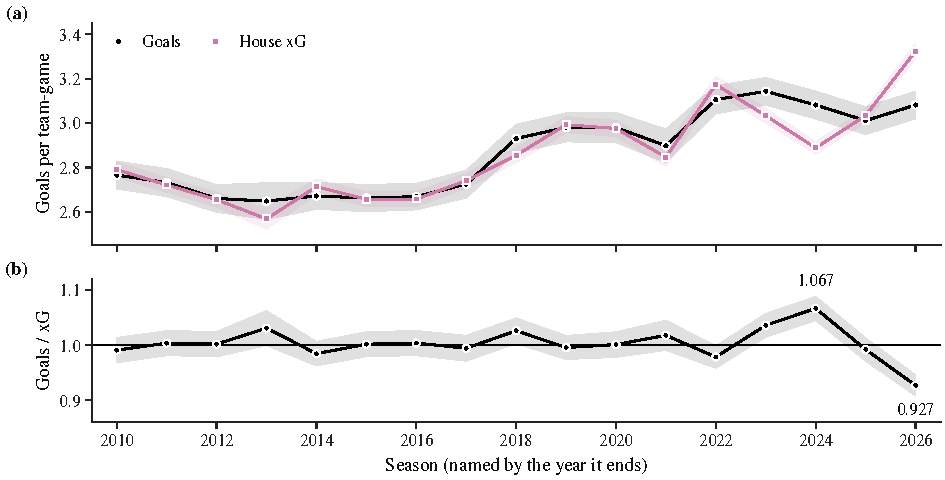
\includegraphics[width=\textwidth]{fig_xg_drift}
\caption{League goals and house expected goals per team-game by season,
all situations except shootouts, with 95\% bands (a), and their ratio (b). The
house expected goals are walk-forward: each season's shots are scored by a model
fitted on earlier seasons with an in-season calibrator that uses only games
already played. The rise in measured expected goals from 2024 to 2026, with
goals flat, follows the change in how shot locations are recorded.}
\label{fig:drift}
\end{figure}

\section{Evaluation protocol}
\label{sec:protocol}

\subsection{Standing rules}

Five rules applied to every model in the project.
\begin{description}[leftmargin=1.2em,style=nextline]
  \item[Vantage.] Anything used to predict a game in season $V$ is computed
  from seasons before $V$ and from games of season $V$ played strictly before
  it: scalers, calibration maps, embeddings, priors and coordinate
  normalisers included. The dressed lineup and the announced starting goalie
  are admissible, because both are public about an hour before the game.
  \item[Market firewall.] No odds or market prices in any feature, target,
  calibration or selection step.
  \item[External models.] Quantities fitted by third parties on full-sample
  data are excluded; only raw recorded fields are admitted.
  \item[Era conditioning.] Era enters through walk-forward covariates (league
  scoring to date, overtime format, shootout and loser-point flags, a scaled
  season index), never through season indicators or full-sample
  normalisation.
  \item[Determinism.] Seeds are fixed and recorded. Neural training runs on
  Apple MPS, which is not bit-deterministic, so each trained checkpoint is
  identified by its SHA-256, every reported number comes from CPU inference
  over a saved checkpoint, and committed per-game predictions must re-derive
  within $10^{-6}$.
\end{description}

\subsection{Windows}

Seasons were assigned to roles before any model was fitted (Table~\ref{tab:data},
Figure~\ref{fig:windows}). For \neurhl{} 1.0 the windows are development
(2009--2011), tune (2012--2017) and confirmation (2018--2026, touched once per
layer), followed by the live 2027 season. Player-level layers use their own
split: development on 2011--2012, tuning on 2014--2017, a declared evaluation
window of 2022--2026 and a one-shot confirmation on 2018--2020. \neurhlG{}, built
after the 1.0 confirmation had spent 2018--2026 at game level, uses a fresh
split of the same history: iteration on 2012 and 2014--2018 (7,421 games),
gates on 2019, 2020 and 2022--2024 (6,289 games), and a sealed test on
2025--2026 (2,624 games). Those seasons had already been scored at game level
by \neurhlH{}, so the \neurhlG{} seal protects against adaptive \neurhlG{} choices; it is
procedurally sealed, not unseen, and we treat the 2026--27 live season as the
only clean test of \neurhlG{}.

The windows are enforced in code. A scoring guard refuses to score an
anomalous season or to cross a window boundary. For \neurhlG{}, a single guarded
loader is the only route by which model, training and evaluation code may
read the data; it drops the sealed seasons unless an unseal function has been
called, and that function refuses every caller except the seal script. A
syntax-tree test fails any \neurhlG{} module that reads the tensor directory
directly, and the 37 sealed input files are pinned by hash.

\begin{figure}[t]
\centering
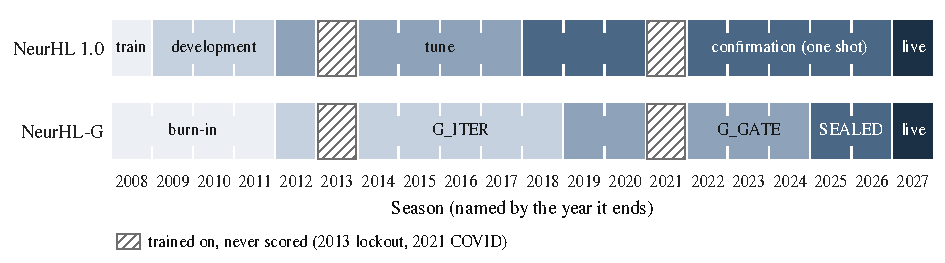
\includegraphics[width=\textwidth]{fig_windows}
\caption{Season roles in the two protocols. \neurhl{} 1.0 spent its
confirmation window, 2018--2026, once per layer. \neurhlG{} reuses the same history
under a new split whose sealed seasons, 2025--2026, remain unspent. Lockout
(2013) and COVID (2021) seasons train but are never scored.}
\label{fig:windows}
\end{figure}

\subsection{Commit before results}

Every plan, amendment and candidate declaration was committed before the
numbers that tested it existed, and every freeze before the confirmatory run it
governs. Amendments are appended, never edited. The repository was not public
before 26 September 2026, so for the plans written before then the ordering
rests on the commit times recorded in its history, which a reader has to take
on trust. From publication on, each push to the public repository is dated
independently of the author: the \neurhlG{} plan and its candidate declaration
were both on the public branch before any \neurhlG{} gate number existed, and
every live forecast must be there before its game starts. Each plan fixes
its gates with numbers, its search budget and the consequence of every
outcome. Searches are logged row by row in ledgers with hard caps: 40
configurations for the first neural game model, 12 for the game-level work of
the second and third plans, 10, 4, 4 and 4 for the player-game, player-season,
goalie and expected-goals layers, and for \neurhlG{} at most 14 full runs on the
iteration window and at most two on the gate window, the second only as one
declared change after a failure. Exceeding a cap voids the version.

Confirmatory tests are one-shot. Each has its own script that refuses to run
before its freeze commit is on the public branch, refuses to run twice, and
writes its result in a single step. A pre-gate on non-confirmatory seasons
decides whether a confirmatory window is spent at all, so a weak candidate
cannot consume it.

\subsection{Causality audits}

Gates that score a model on the inputs it was trained with cannot detect an
illegitimate input: a leaked feature improves in-sample realism along with
everything else (Section~\ref{sec:failures}). Every data builder therefore
passes a causality audit before any gated number is reported from its output.
The audit corrupts every row after a cut date, rebuilds the features, and
requires every value before the cut to be bit-identical. For the event
simulator the same test runs at the level of individual model inputs, together
with a target-identity check (no input may agree with any target above 98\%)
and an empirical check that exempted inputs carry no lift on the next event.
The \neurhlG{} state builders are audited the same way, with cuts in mid-season
2016 and at the boundary between the last gate season and the first sealed
one; all 100 skater-state, 23 goalie-state and 53 team-state features are
bit-identical before each cut.

\subsection{Statistics}

The primary metric for win probabilities is per-game log loss, compared
between models as a mean paired difference over the same games. We report a
normal-approximation test on the per-game differences, a season-clustered $t$
test, a wild cluster bootstrap on seasons that enumerates all $2^S$
Rademacher sign patterns exactly, a moving-block bootstrap over date-ordered
games (blocks of 100 games, 9,999 draws, seed 711), a sign test across
seasons, and the Murphy decomposition of the Brier score into reliability,
resolution and uncertainty. A log-loss gain with no gain in resolution is
reported as recalibration, not information. Player-level differences use
standard errors clustered two ways, by player and by game
\citep{cameron2011robust}, and families of tests are Holm-corrected. Count
predictions are assessed with Poisson deviance, the continuous ranked
probability score and randomised probability integral transforms.

Power is stated before each test. On the tune window, one standard error of a
paired log-loss difference against Elo is 0.00268 nats. A gate of the form
``beat Elo by 0.002'' is therefore a 0.75-standard-error bar, which a model
with no skill clears by chance 23\% of the time. The first plan's second
amendment made a significance test the headline criterion for exactly this
reason, and every later plan kept it.

\section{Models}
\label{sec:models}

Figure~\ref{fig:overview} shows how the components fit together. All of them
are walk-forward: the model that predicts season $T$ is fitted on seasons
before $T$ only.

\begin{figure}[t]
\centering
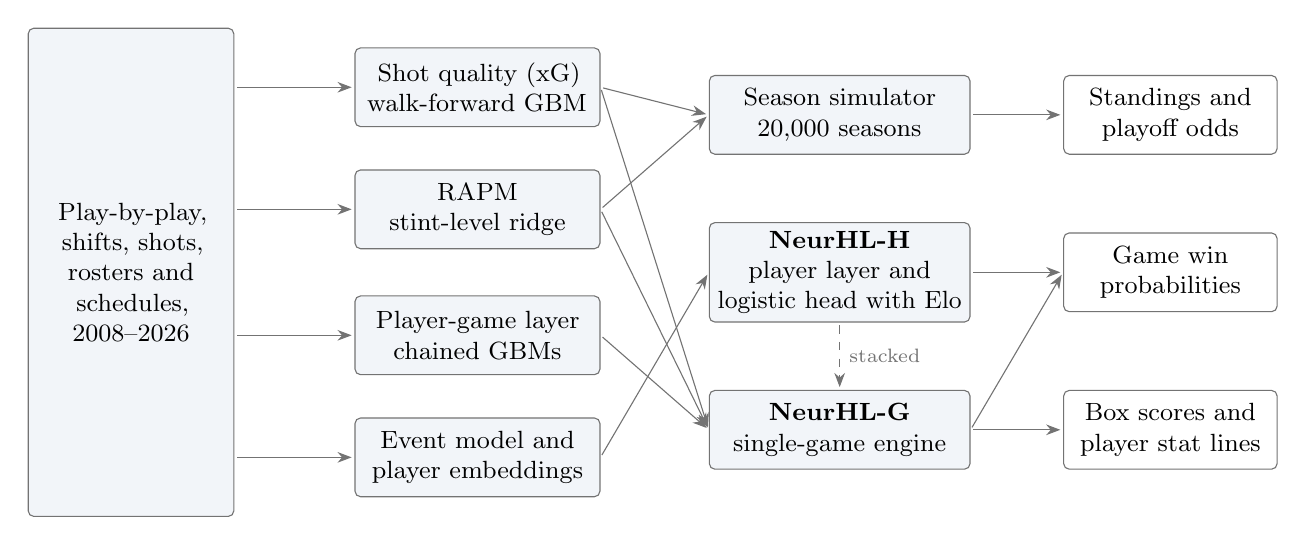
\begin{tikzpicture}[
  font=\small,
  comp/.style={draw=black!55, fill=boxfill, rounded corners=2pt, align=center,
               minimum height=10mm, inner sep=3pt, text width=#1},
  comp/.default=29mm,
  res/.style={draw=black!55, fill=white, rounded corners=2pt, align=center,
              minimum height=10mm, inner sep=3pt, text width=25mm},
  arr/.style={-{Stealth[length=1.8mm]}, black!55, shorten >=1pt, shorten <=1pt}]
\node[comp=24mm, minimum height=62mm] (raw) at (0,0) {Play-by-play,\\shifts, shots,\\rosters and\\schedules,\\2008--2026};
\node[comp] (xg)   at (4.4, 2.35)  {Shot quality (xG)\\walk-forward GBM};
\node[comp] (rapm) at (4.4, 0.8)   {RAPM\\stint-level ridge};
\node[comp] (pg)   at (4.4, -0.8)  {Player-game layer\\chained GBMs};
\node[comp] (emb)  at (4.4, -2.35) {Event model and\\player embeddings};
\node[comp=31mm] (season) at (9.0, 2.0)  {Season simulator\\20,000 seasons};
\node[comp=31mm] (h)      at (9.0, 0.0)  {\textbf{\neurhlH{}}\\player layer and\\logistic head with Elo};
\node[comp=31mm] (g)      at (9.0, -2.0) {\textbf{\neurhlG{}}\\single-game engine};
\node[res] (o1) at (13.2, 2.0)  {Standings and\\playoff odds};
\node[res] (o2) at (13.2, 0.0)  {Game win\\probabilities};
\node[res] (o3) at (13.2, -2.0) {Box scores and\\player stat lines};
\foreach \n in {xg, rapm, pg, emb} \draw[arr] (raw.east |- \n) -- (\n.west);
\draw[arr] (xg.east) -- (season.west);
\draw[arr] (rapm.east) -- (season.west);
\draw[arr] (emb.east) -- (h.west);
\draw[arr] (xg.east) -- (g.west);
\draw[arr] (rapm.east) -- (g.west);
\draw[arr] (pg.east) -- (g.west);
\draw[arr, dashed] (h.south) -- node[right, font=\scriptsize] {stacked} (g.north);
\draw[arr] (season.east) -- (o1.west);
\draw[arr] (h.east) -- (o2.west);
\draw[arr] (g.east) -- (o3.west);
\draw[arr] (g.east) -- (o2.west);
\end{tikzpicture}

\caption{Components of \neurhl{}, each fitted walk-forward. RAPM and expected
goals feed the season simulator and \neurhlG{}'s priors and rates; the event
model's player embeddings feed \neurhlH{}; the player-game layer gives
\neurhlG{} its baselines and, summed over the schedule, the player season
projections. \neurhlG{}'s final win probability stacks its own output with
\neurhlH{} and Elo.}
\label{fig:overview}
\end{figure}

\subsection{Baselines}
\label{sec:m-elo}

The primary comparator is the house Elo system (``v1''), tuned on 2006--2017
before any \neurhl{} work began. Before each game with ratings $r_h$ and $r_a$
and home advantage $H$, the expected home score is
\begin{equation}
E_h = \bigl(1 + 10^{-(r_h + H - r_a)/400}\bigr)^{-1}.
\end{equation}
After the game both ratings move by $\pm K M (y - E_h)$, where $y$ is the home
result and $M = \ln(|\Delta g| + 1)\cdot 2.2 / (2.2 + 0.001\,d_w)$ is a
margin-of-victory multiplier that shrinks with the winner's rating advantage
$d_w$. Between seasons each rating regresses toward the mean,
$r \leftarrow \mu + \phi (r - \mu)$. The frozen parameters are $K = 6$,
$H = 35$ and $\phi = 0.7$. Game probabilities come from walk-forward logistic
models of the rating difference: the probability of reaching overtime, the
regulation winner, and the overtime or shootout winner. We also report a
constant home-win rate, and ``Tier-0'', the stronger of a standardised
logistic regression and an early-stopped gradient-boosted model
\citep{chen2016xgboost} on 23
engineered game features (Elo difference, rest, travel, goalie form, roster
aggregates, era), which scored 0.67692 on 2014--2017 against Elo's 0.67548.

\subsection{Shot quality}
\label{sec:m-xg}

The expected-goals model is a histogram gradient-boosted classifier
\citep{friedman2001greedy,ke2017lightgbm} (400
iterations, learning rate 0.06, 31 leaves, at least 200 shots per leaf, L2
penalty 1.0, early stopping) on 33 features: distance and angles, rebound and
rush indicators, the previous event's type, distance, angle and elapsed time,
speed from the previous event, strength state and empty nets, score
difference, period, shooter handedness and position, shot type, and
walk-forward era and rink covariates. For vantage $V$ the model is fitted on
seasons before $V-1$. Its calibration map is isotonic, refitted every 25 league
games on the most recent 120,000 out-of-sample shots strictly before the game
being scored, so it follows the recording drift with the data in which the
drift occurs. The model beats a distance-and-angle logistic regression in all
18 vantages (gate X1), and team expected-goal differential predicts future goal
share better than shot-attempt (Corsi) differential across 554 team-seasons,
$r = 0.423$ against $0.395$ (gate X2). It fails its calibration gate X3, a
maximum deviation of 0.005 per decile, at 0.0065 after three declared
correction ladders; the residual is concentrated in the top decile in the
seasons of the recording change.

\subsection{Adjusted plus-minus}
\label{sec:m-rapm}

RAPM is a stint-level ridge regression \citep{hoerl1970ridge} of on-ice shot rates on indicator
columns for the players on the ice, with an intercept, a home term and
unpenalised team-season fixed effects, so that player coefficients measure
performance relative to the player's own team. The penalty, $\lambda = 51{,}200$,
is chosen to maximise how well a prior rating predicts a player's realised
on-ice results after he changes team. RAPM priors are computed as of each
season and feed the season simulator and \neurhlG{}.

\subsection{Event simulator}
\label{sec:m-events}

The event simulator is a Transformer-Hawkes marked temporal point process
\citep{zuo2020transformer} over the unified event and line-change stream, with
heads for the time to the next event, its type and team, location, zone and
actor, and player effects entering as zero-initialised modulations of the
hazard anchored on RAPM, in the spirit of \citet{thomas2013competing}. It has
5.3 million parameters and is trained as a five-seed ensemble. After the two
leaks described in Section~\ref{sec:failures} were removed it reproduces goals,
shots, penalties and faceoffs per game and per period within 10\% of observed
rates, and its score effects match observed ones with a gradient ratio of
0.979. Its score-effect curve initialises the \neurhlG{} hazard table.

\subsection{Player-game layer}
\label{sec:m-pg}

The player-game layer predicts, for every dressed skater, his share of team
ice time, his shots on goal, and the probabilities of scoring at least one goal
and recording at least one assist. It chains four histogram gradient-boosted
models in the order opportunity, volume, conversion: predicted usage feeds the
shot model, and both feed the two binary models. Declared feature blocks cover
the player's own recent form (the baseline's inputs, nested), usage structure
by strength, line rank and power-play unit, opportunity created by absent
teammates, opponent and schedule context, and line and coaching patterns.
Binary heads are calibrated isotonically on the previous season's
out-of-sample predictions, and ice-time shares are renormalised within each
team-game so they sum to one exactly.

\subsection{Season simulator and player seasons}
\label{sec:m-season}

The season simulator integrates team scoring rates, roster RAPM and score
effects over each game of the real schedule and simulates 20,000 seasons,
drawing each team's strength once per simulated season ($\sigma = 0.07$) so that
uncertainty about how good a team is persists through the season. Player
season projections blend a gradient-boosted season model with the
player-game layer summed over the schedule under an availability hazard,
50/50, the combination a declared rule selected.

\subsection{\neurhlH{}}
\label{sec:m-h}

\neurhlH{} has three layers. Layer~1 predicts what each player will do in a game:
his on-ice shot attempts for and against per 60 minutes, close-range attempts
for and against, and his ice time. It is residual on the player's own
exponentially weighted history: a two-hidden-layer network (128 units, GELU,
dropout 0.1) maps a 64-dimensional player embedding from the event model, 13
static features (position, age and age squared, career games, games with the
current team, a recent-move flag, home, rest, team game number, games played
this season, a late-season flag) and six history features to multiplicative
corrections bounded by $\pm 0.7$ in log space, with a zero-initialised output
layer so that training starts at the baseline. It is trained walk-forward on
about 750,000 player-games. Layer~2 aggregates the predictions over the
players actually dressed, weighted by predicted ice time, into team
projections: projected attempt share and close-range share. Layer~3 is a thin
head, a standardised logistic regression on four inputs, the Elo logit, the
projected attempt-share difference, the projected close-range difference and
the rest difference, refitted for each season on all earlier seasons. Its
regularisation constant is selected on training loss, a known weakness that
favours weak regularisation; it was kept verbatim for the confirmation because
changing it would have tested a different model.

\subsection{\neurhlG{}}
\label{sec:m-g}

\neurhlG{} predicts one game from the two dressed lineups and simulates its box
score. Figure~\ref{fig:g-arch} summarises the architecture.

\paragraph{State.}
After every game each skater's state is updated by discounted sums of his
per-game statistics with per-game decays 0.98, 0.95, 0.85 and 0.60. Rates are
ratios of discounted sums, reported with their effective sample sizes, beside
season-to-date and career totals and as-of priors (the RAPM prior and the
event-model embedding fitted on earlier seasons only). The 114 skater features
cover ice time by strength, individual shots, attempts and expected goals,
goals, assists, on-ice expected goals for and against, and penalties. Goalie
state (23 features) includes shrunk save percentage, goals saved above
expected per expected goal, and workload. Team state (57 features) holds
discounted team rates, and context (10 features) holds the Elo logit, rest,
travel, time-zone change and era covariates. A game late in a season therefore
sees every earlier game of that season as well as all earlier seasons.

\paragraph{Network.}
Shared encoders map each skater (114 features plus position, $\to 128 \to 64$),
each team ($57 \to 64 \to 32$), each goalie ($23 \to 32 \to 16$) and the context
($10 \to 32 \to 16$), each a linear layer, GELU, layer normalisation, dropout
0.2 and a linear layer. Heads produce residual corrections with
zero-initialised output layers: 12 per skater (ice time by strength, shot,
attempt and expected-goal propensities, finishing, playmaking, offensive and
defensive on-ice effects, penalties drawn and taken), six per team and one per
goalie. The untrained network therefore reproduces shrunk-history baselines
exactly. The model has 48,810 parameters.

\paragraph{Team layer.}
The team layer is deterministic and conserves ice time. With $o$ the opponent
of side $s$, power-play opportunities have mean
$\lambda^{pp}_s = \mathrm{log5}(\text{drawn}_s, \text{taken}_o)\,e^{\delta_s}$,
where $\mathrm{log5}(a, b) = ab/L$ for league rate $L$ \citep{hammond2015james}, and $\delta_s$ collects
the skaters' penalty terms. Power-play time is $T^{pp}_s = \tau \lambda^{pp}_s$,
short-handed time is the opponent's power-play time, and even-strength time is
$T^{ev} = 60 - T^{pp}_s - T^{pp}_o$ minutes. Player $i$'s ice time at strength
$k$ is
\begin{equation}
\mathrm{TOI}_{ik} = n_k\, T^{k}\, \mathrm{softmax}_{j \in \mathcal{P}(i)}\bigl(b_{jk} + \delta_{jk}\bigr)_i,
\end{equation}
a softmax over the player's position group $\mathcal{P}(i)$ with $n_k$ players on
the ice (three forwards and two defence at even strength, five skaters on the
power play, four short-handed), so team ice time is exact by construction.
Team scoring rates are log-linear:
\begin{equation}
\log r^{ev}_s = \log \mathrm{log5}\bigl(\mathrm{xGF60}_s, \mathrm{xGA60}_o\bigr)
  + \sum_{i \in s} w_i\, \mathrm{off}_i - \sum_{j \in o} w_j\, \mathrm{def}_j + \delta^{tm}_s,
\end{equation}
where $w$ are ice-time weights and the team rates are shrunk toward league
values by their effective sample sizes. Player shots, attempts, expected goals,
goals, assists and on-ice expected goals are softmax allocations of team
totals, so they sum exactly, and team goals are expected goals times a
finishing term less the opposing goalie's effect.

\paragraph{Outcome.}
Win probabilities come from a differentiable integration over the goal
differential, a Markov chain in the spirit of \citet{kaplan2014markov}. Let $\lambda_h, \lambda_a$ be the two regulation scoring rates. The
distribution of the differential $d \in \{-8, \dots, 8\}$ evolves over 30 steps of
two minutes. In each step side $s$ scores with probability
$q_s = 1 - \exp\{-\lambda_s e^{u}\,\Delta t\, e^{\eta(\ell_s, \pi)}\}$, where
$\ell_s \in \{-3, \dots, 3\}$ is the side's own lead (clamped), $\pi$ indexes five
game phases (minutes 0--40, 40--50, 50--56, 56--58, 58--60), and $\eta$ is a
learned $7 \times 5$ hazard table initialised from the event simulator's score
effects \citep[compare][]{thomas2013competing}. Trailing teams push, leaders
sit back, tied teams turn cautious late, and the last minutes capture pulled
goalies. The pace shock
$u = \sqrt{2}\,\sigma x - \sigma^2/2$ is shared by both teams and integrated with
five-node Gauss--Hermite quadrature \citep{abramowitz1964handbook}, which supplies the tie mass by mechanism
rather than through an ad hoc scalar. The probability of a regulation tie is
the mass at $d = 0$, and the overtime or shootout winner is a logistic function
of $\log(\lambda_h/\lambda_a)$. The output is the four-way outcome: home or away
win, in regulation or after it.

\paragraph{Training.}
Snapshot $T$ is trained on seasons 2009 through $T-1$. Phase~1 minimises
Huber losses on ice time by strength and on power-play minutes, Poisson
deviances on skater and team counts, and the four-way outcome negative log
likelihood with weight 0.3 (AdamW \citep{loshchilov2019decoupled}, learning rate $2\times10^{-3}$, weight decay
0.01, one-cycle schedule, batches of 256 games, 10 epochs). Phase~2 raises
the outcome weight to 1 and trains four more epochs at learning rate
$3\times10^{-4}$, with an L2-SP penalty \citep{li2018explicit} of $10^{-3}$
toward the phase-1 weights. The ensemble averages five seeds.

\paragraph{Final probability.}
For each season $T$ a logistic stack \citep{wolpert1992stacked} over the Elo logit, the \neurhlG{} logit and
the \neurhlH{} logit is fitted on out-of-sample predictions from earlier seasons.
The column subset, which always includes Elo, is chosen by leave-one-season-out
cross-validation on the training seasons, with a fallback to Elo and \neurhlG{}
where \neurhlH{} is unavailable.

\paragraph{Stat sheet.}
Box scores are simulated 10,000 times per game and are consistent with the
win probability by construction. Each draw samples the outcome category from
the stacked four-way probabilities, then a regulation score conditional on it,
then team shots (negative binomial around the model mean, $r = 40$, floored at
goals), team expected goals (gamma), power-play opportunities (Poisson),
player shots and goals (multinomial splits by the model's shares), assists
(zero, one or two per goal in the league's typical mix, split by assist
shares), individual expected goals (Dirichlet split) and goalie saves.

\begin{figure}[t]
\centering
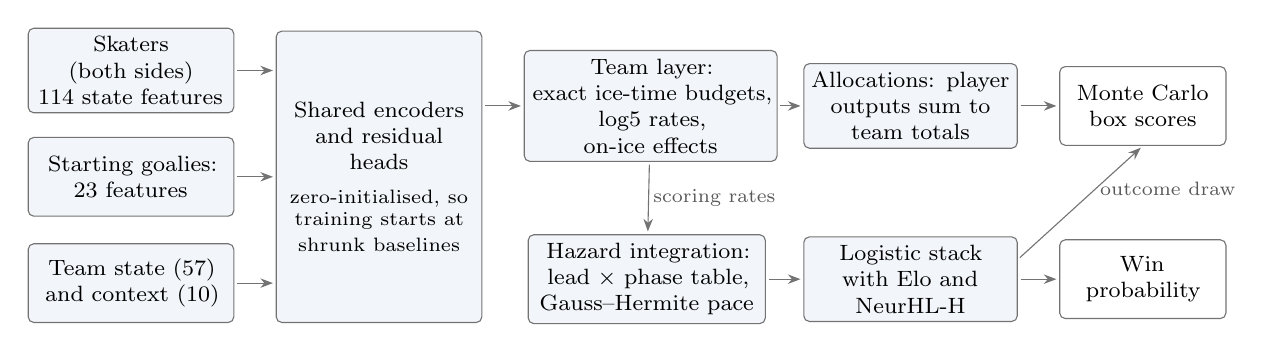
\begin{tikzpicture}[
  font=\footnotesize,
  every node/.append style={execute at begin node={\hyphenpenalty=10000\exhyphenpenalty=10000}},
  b/.style={draw=black!55, fill=boxfill, rounded corners=2pt, align=center,
            minimum height=10mm, inner sep=3pt, text width=#1},
  b/.default=25mm,
  o/.style={draw=black!55, fill=white, rounded corners=2pt, align=center,
            minimum height=10mm, inner sep=3pt, text width=19mm},
  arr/.style={-{Stealth[length=1.6mm]}, black!55, shorten >=1pt, shorten <=1pt},
  lab/.style={font=\scriptsize, text=black!65, inner sep=1.5pt}]
\node[b=24mm] (sk) at (0, 1.35)  {Skaters (both sides)\\114 state features};
\node[b=24mm] (gk) at (0, 0)     {Starting goalies:\\23 features};
\node[b=24mm] (tm) at (0, -1.35) {Team state (57)\\and context (10)};
\node[b=24mm, minimum height=37mm] (enc) at (3.15, 0) {Shared encoders\\and residual heads\\[4pt]{\scriptsize zero-initialised, so\\training starts at\\shrunk baselines}};
\node[b=30mm] (team) at (6.6, 0.9) {Team layer:\\exact ice-time budgets,\\log5 rates, on-ice effects};
\node[b=25mm] (alloc) at (9.9, 0.9) {Allocations: player\\outputs sum to\\team totals};
\node[o] (mc) at (12.85, 0.9) {Monte Carlo\\box scores};
\node[b=28mm] (haz) at (6.55, -1.3) {Hazard integration:\\lead $\times$ phase table,\\Gauss--Hermite pace};
\node[b=25mm] (stk) at (9.9, -1.3) {Logistic stack\\with Elo and \neurhlH{}};
\node[o] (wp) at (12.85, -1.3) {Win\\probability};
\foreach \n in {sk, gk, tm} \draw[arr] (\n.east) -- (enc.west |- \n);
\draw[arr] (enc.east |- team) -- (team.west);
\draw[arr] (team) -- (alloc);
\draw[arr] (alloc) -- (mc);
\draw[arr] (team) -- node[lab, right] {scoring rates} (haz);
\draw[arr] (haz) -- (stk);
\draw[arr] (stk) -- (wp);
\draw[arr] (stk.east) ++(0,2.5mm) -- node[lab, pos=0.62, right] {outcome draw} (mc.south);
\end{tikzpicture}

\caption{\neurhlG{}. Encoders and residual heads adjust shrunk-history baselines; a
deterministic team layer conserves ice time and makes player outputs sum to
team totals; a hazard integration over the goal differential gives the
four-way outcome, which is stacked with Elo and \neurhlH{}; box scores are
simulated conditional on the stacked outcome.}
\label{fig:g-arch}
\end{figure}

\section{Results}
\label{sec:results}

We report confirmed results first, then the \neurhlG{} gate evidence, then the
development-only season results and the null results. A result is
\emph{confirmed} only if it came from a window no decision had used, scored
once after the model was frozen. Results from windows that were consulted
during development are \emph{exploratory}.

\subsection{Confirmed: the player-game layer}
\label{sec:res-pg}

The player-game layer was frozen after development and scored once on the
player confirmation window, 2018--2020: 130,092 skater-games by 1,152 players in
3,624 games. The comparator is each skater's own recent history: an
exponentially weighted average ($\alpha = 0.1$) for ice-time share and shots,
renormalised over the dressed skaters, and for the two binary targets a
walk-forward shrunk average $\hat p = (n\,\bar x + k\,p_0)/(n + k)$ \citep{efron1975data}
with $k$ chosen on the previous season. This is a demanding baseline: in the first plan a neural
player-rate model had lost to it on ice time and shots (Table~\ref{tab:nulls}).
Table~\ref{tab:pg} shows the result. The layer is better on all four targets,
in every season, with two-way clustered $z$ statistics between $-8.1$ and
$-23.9$ and Holm-adjusted $p < 10^{-5}$.

\begin{table}[t]
\centering
\small
\caption{Player-game layer against each skater's own recent history on the
one-shot player confirmation, 2018--2020 (130,092 skater-games). Relative
difference in the stated loss; negative is better. $z$ uses standard errors
clustered by player and by game.}
\label{tab:pg}
\begin{tabular}{llrrc}
\toprule
Target & Loss & Relative difference & $z$ (two-way) & Seasons better \\
\midrule
Ice-time share & MAE & $-4.1\%$ & $-23.9$ & 3/3 \\
Shots on goal & Poisson deviance & $-10.2\%$ & $-13.7$ & 3/3 \\
P(goal $\geq 1$) & log loss & $-2.8\%$ & $-8.1$ & 3/3 \\
P(assist $\geq 1$) & log loss & $-2.6\%$ & $-15.9$ & 3/3 \\
\bottomrule
\end{tabular}
\end{table}

\subsection{Confirmed: \neurhlH{} against Elo}
\label{sec:res-h}

\neurhlH{} was frozen exactly as it had been evaluated on the tune window, the
freeze and the test were committed in an amendment before any 2018--2026 game
was scored by any \neurhlH{} artifact, and the test ran once. The primary set is
the eight structurally normal seasons of 2018--2026 ($n = 10{,}184$ games; 2021
excluded). Table~\ref{tab:c1} and Figure~\ref{fig:c1} give the results.

\begin{table}[t]
\centering
\small
\caption{One-shot confirmation of \neurhlH{} against Elo, regular-season games of
2018--2026 excluding 2021 ($n = 10{,}184$). Differences are \neurhlH{} minus Elo in
per-game log loss; negative favours \neurhlH{}.}
\label{tab:c1}
\begin{tabular}{lr}
\toprule
Quantity & Value \\
\midrule
Log loss, \neurhlH{} / Elo & 0.66495 / 0.66973 \\
Mean paired difference (SE) & $-0.00478$ (0.00088) \\
95\% CI, normal / moving-block bootstrap & \ci{-0.00650}{-0.00306} / \ci{-0.00660}{-0.00293} \\
Per-game test & $z = -5.46$, $p < 10^{-6}$ \\
Season-clustered $t$ (7 df) & $t = -5.71$, $p = 0.0007$ \\
Wild cluster bootstrap, exact ($2^8$ patterns) & $p = 0.0078$ \\
Seasons better; sign test & 8 of 8; $p = 0.0078$ \\
Including 2021 ($n = 11{,}052$) & $-0.00459$ \ci{-0.00622}{-0.00295}, 9 of 9 \\
\midrule
Brier score, \neurhlH{} / Elo & 0.23630 / 0.23857 \\
Reliability, \neurhlH{} / Elo & 0.00021 / 0.00025 \\
Resolution, \neurhlH{} / Elo & 0.01218 / 0.00982 \\
Uncertainty & 0.24840 \\
\bottomrule
\end{tabular}
\end{table}

\begin{figure}[t]
\centering
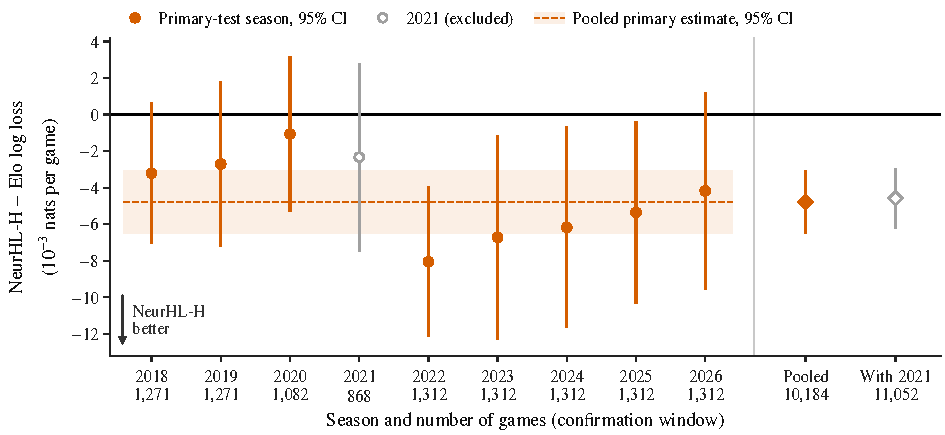
\includegraphics[width=\textwidth]{fig_c1_seasons}
\caption{\neurhlH{} minus Elo, per-game log loss by season on the one-shot
confirmation, with 95\% intervals; negative favours \neurhlH{}. Numbers under
the season labels are games. 2021 (hollow) is excluded from the primary test by
the declared rule and shown for completeness. The band and filled diamond are
the pooled primary estimate; the hollow diamond pools all nine seasons.}
\label{fig:c1}
\end{figure}

The effect is $-0.00478$ nats per game (95\% CI $-0.00650$ to $-0.00306$), and it
holds in every season. It is also the size the tune window had suggested
($-0.00283$), somewhat larger rather than smaller, and the amendment's power
table had put the chance of detecting an effect of the tune-window size at
about 0.93. Measured against a constant equal to the window's home-win rate
(0.540, log loss 0.68995), Elo's skill is 0.0202 nats and \neurhlH{}'s is 0.0250, an
increase of about 24\%. The Murphy decomposition locates the gain: reliability
is essentially unchanged and already small for both models, while resolution
rises from 0.0098 to 0.0122. \neurhlH{} is not a recalibrated Elo; it separates
games that Elo treats alike. Figure~\ref{fig:reliability} shows that both
models are well calibrated across the probability range.

The gain is conditional on information Elo does not use. \neurhlH{} reads which
skaters dressed for each game, which is public about an hour before puck drop,
and its Layer~1 translates those players' histories and career context into
projected shot shares. The confirmation therefore establishes that lineup-level
player information improves on a strong team-level rating system, not that a
network discovers team strength that Elo misses.

\paragraph{Where the gain comes from (exploratory).}
To test whether the lineup is what \neurhlH{} adds, we split the confirmation
games after the fact by how lopsided the two teams' absences were: the recent
ice time of regulars who did not dress, home minus away, in minutes. The window
is spent, so this analysis is exploratory. Its script stated two expectations
before it ran: that the gain would grow with the imbalance, and that it would
be largest early in the season, when rosters have changed and Elo has not yet
seen them play. The first held and the second did not (Table~\ref{tab:gain}).
Where neither team was missing regular ice time the difference is $-0.0003$
(SE 0.0045); it grows to $-0.0087$ when the imbalance exceeds 40 minutes, a
slope of $-0.0010$ per 10 minutes (SE 0.0004). By month the gain is smallest
in October and November and largest from December on. \neurhlH{} does not move
further from Elo when absences are lopsided (the mean absolute difference
between the two probabilities is 0.034 to 0.036 in every bin); its adjustments
are simply more accurate there.

\begin{table}[t]
\centering
\small
\caption{\neurhlH{} minus Elo, per-game log loss on the confirmation games,
split after the fact by the imbalance in absent regulars' recent ice time
between the two teams, and by month. Exploratory: the window had been spent.}
\label{tab:gain}
\begin{tabular}{lrr@{\hspace{2.5em}}lrr}
\toprule
Absence imbalance & Games & Difference (SE) & Month & Games & Difference (SE) \\
\midrule
none & 367 & $-0.0003$ (0.0045) & October & 1,316 & $-0.0017$ (0.0023) \\
0--20 min & 4,747 & $-0.0029$ (0.0013) & November & 1,726 & $-0.0022$ (0.0021) \\
20--40 min & 2,928 & $-0.0055$ (0.0016) & December & 1,674 & $-0.0078$ (0.0021) \\
over 40 min & 2,142 & $-0.0087$ (0.0020) & January & 1,600 & $-0.0057$ (0.0023) \\
 & & & February & 1,318 & $-0.0061$ (0.0024) \\
 & & & March & 1,712 & $-0.0042$ (0.0022) \\
 & & & April & 837 & $-0.0061$ (0.0032) \\
\bottomrule
\end{tabular}
\end{table}

\begin{figure}[t]
\centering
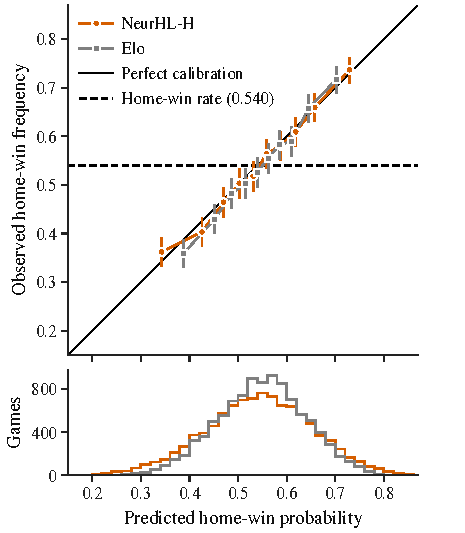
\includegraphics[width=0.62\textwidth]{fig_reliability}
\caption{Reliability of \neurhlH{} and Elo on the 10,184 confirmation games: ten
equal-count bins per model with 95\% Wilson intervals, the diagonal of perfect
calibration and the observed home-win rate (dashed); below, the distribution of
predicted home-win probabilities. \neurhlH{} spreads its forecasts more widely
while staying on the diagonal.}
\label{fig:reliability}
\end{figure}

\subsection{\neurhlG{}: iteration, gates and the pre-gate}
\label{sec:res-g}

\paragraph{Iteration.}
Table~\ref{tab:ladder} and Figure~\ref{fig:ladder} give the ladder on the
iteration window, every run of which is in the search ledger. The non-neural
engine (player-game sums through the integration and the stack) and the
tree-based rung did no better than Elo. The network with official power-play
targets (R6) improved on Elo by 0.0023 but did not reach \neurhlH{}. None of four
additions earned its place under the declared adoption rule (a gain of at
least 0.0003 without losing in four or more of six seasons): an Elo anchor on
the scoring rates, lineup-versus-usual multipliers, \neurhlH{}'s projections as
team inputs, and attention across the two rosters. Stacking R6 with \neurhlH{}
(R11) gave the best stack, 0.67258, still 0.00014 behind \neurhlH{} alone. The
paired standard error of each rung's difference from \neurhlH{} is 0.0007 to
0.0009, larger than most gaps between rungs, so the ladder shows the absence of
a large gain rather than a reliable ordering. The candidate declared for the
gate, g1, is R11 with the five-seed ensemble. The
candidate commit recorded, before the gate ran, the expectation that the
pre-gate would fail.

\begin{table}[t]
\centering
\small
\caption{\neurhlG{} iteration ladder on 2012 and 2014--2018 (7,421 games): pooled
log loss of each rung's final probability, from the search ledger. R4 was run
on the quick protocol (two seasons, 2,501 games), so its value is on a
different set of games. R6e and R6L were run before the master tensor was
rebuilt on official power-play opportunities; their parent on the earlier
tensor scored 0.67299, against which R6e is $+0.00031$ and R6L $-0.000004$, so
neither decision depends on the version.}
\label{tab:ladder}
\begin{tabular}{llr}
\toprule
Rung & Change & Log loss \\
\midrule
R1 & Elo & 0.67528 \\
R2 & \neurhlH{} & 0.67244 \\
R3 & gradient-boosted trees / logistic on game features, Elo-stacked & 0.67611 / 0.69699 \\
R4 & non-neural engine (quick protocol) & 0.67581 \\
R6 & network, official power-play targets & 0.67301 \\
R6e & + Elo anchor on scoring rates & 0.67330 \\
R6L & + lineup-versus-usual multipliers & 0.67299 \\
R6c & + \neurhlH{} projections as team inputs & 0.67344 \\
R13 & R6c + direct \neurhlH{} terms & 0.67344 \\
R9 & R6c + attention across rosters & 0.67366 \\
R11 & R6 stacked with \neurhlH{} (candidate structure) & 0.67258 \\
\bottomrule
\end{tabular}
\end{table}

\begin{figure}[t]
\centering
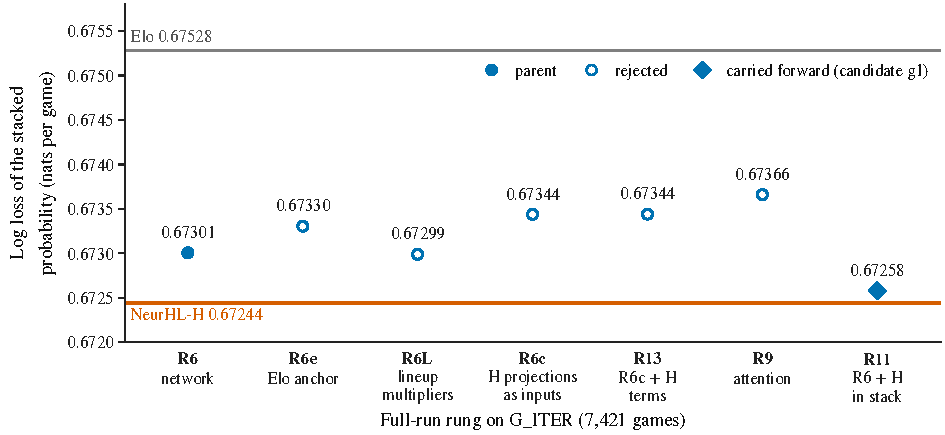
\includegraphics[width=\textwidth]{fig_g_ladder}
\caption{\neurhlG{} iteration ladder: pooled log loss of each full-run rung on the
iteration window (7,421 games), with Elo and \neurhlH{} on the same games. Open
circles were rejected under the adoption rule; the filled diamond, R11, was
carried forward as the candidate.}
\label{fig:ladder}
\end{figure}

\paragraph{Gates.}
The candidate was scored once on the gate window (6,289 games).
Table~\ref{tab:gates} summarises the gates and Figure~\ref{fig:gate} the
per-season differences. The final probability beats Elo by 0.00559 nats (SE
0.00131), in all five seasons, a margin comparable to \neurhlH{}'s confirmed one. It
beats \neurhlH{} by only 0.00049 (SE 0.00060), in three of five seasons. The
pre-gate required both a gain of at least 0.0045 over Elo and a gain of at
least 0.0010 over \neurhlH{}, each in at least four of five seasons. The first
condition holds and the second does not, so the pre-gate failed and, as the
plan declared, the sealed seasons were not spent. At the sealed test's size the
minimum detectable effect at 80\% power would have been 0.0057 against Elo and
0.0026 against \neurhlH{}.

\begin{table}[t]
\centering
\small
\caption{\neurhlG{} (candidate g1) on the gate window, 2019, 2020 and 2022--2024
(6,289 games; 225,752 skater-games). The calibration row reflects the
correction in Section~\ref{sec:failures}.}
\label{tab:gates}
\begin{tabular}{p{0.34\textwidth}p{0.56\textwidth}}
\toprule
Gate & Result \\
\midrule
Final probability vs Elo & $-0.00559$ (SE 0.00131), 5 of 5 seasons \\
Final probability vs \neurhlH{} & $-0.00049$ (SE 0.00060), 3 of 5 seasons \\
Pre-gate (S-STOP) & \textbf{fail}: the \neurhlH{} condition is not met \\
\midrule
PG: player heads vs the player-game layer & pass: ice-time share $-0.59\%$, shots $-0.45\%$ (Poisson log loss), P(goal) $-0.45\%$, P(assist) $-0.36\%$; every upper 95\% bound below zero (two-way clustered) \\
T: team box score & pass: shots, expected goals, goals and power-play opportunities beat log5 team history; shots and goals also beat the summed player-game layer, on deviance and CRPS \\
C: calibration & \textbf{fail}: slope 0.968 and overtime share (0.224 predicted, 0.220 observed) pass; randomised-PIT 80\% coverage passes for team goals (0.803) and skater shots (0.783) but not for team shots (0.860) \\
\bottomrule
\end{tabular}
\end{table}

\begin{figure}[t]
\centering
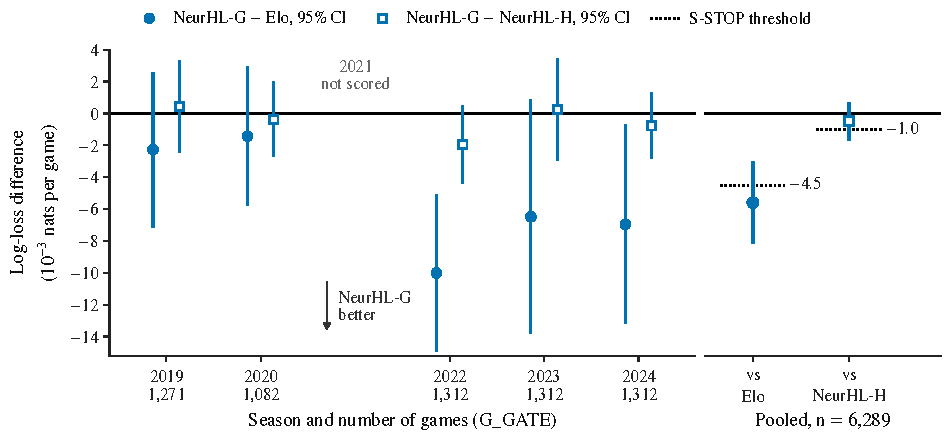
\includegraphics[width=\textwidth]{fig_g_gate_seasons}
\caption{\neurhlG{} on the gate window: per-season differences in per-game log loss
of the final probability against Elo (filled) and against \neurhlH{} (open), with
95\% intervals, and the pooled estimates over 6,289 games. Dotted segments mark
the pre-gate thresholds, $-0.0045$ against Elo and $-0.0010$ against \neurhlH{}.}
\label{fig:gate}
\end{figure}

\paragraph{The stat sheet.}
The engine's player heads improve on the confirmed player-game layer on all
four shared targets (Figure~\ref{fig:heads}). The gains are small, between
0.36\% and 0.59\%, but every upper confidence bound is below zero. Its team box
scores beat both declared baselines. Binned predictions track outcomes closely
for shots; for expected goals and goals they are somewhat too spread at the
extremes, so that the decile with the highest predicted regulation goals (4.2
per team-game) averaged 3.7 (Figure~\ref{fig:teambox}). The
win-probability slope is 0.968, and the hazard integration reproduces the
share of games that go past regulation without a tie scalar (22.4\% predicted
against 22.0\% observed; Figure~\ref{fig:otcal}). One calibration check fails:
the negative-binomial dispersion used for team shots makes those intervals too
wide, covering 86\% of outcomes at a nominal 80\%.

\begin{figure}[t]
\centering
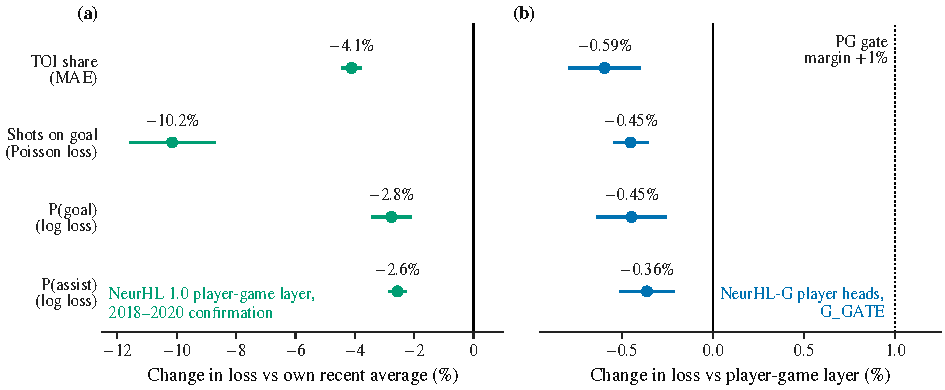
\includegraphics[width=\textwidth]{fig_player_heads}
\caption{Relative change in loss of player-level predictions, with 95\%
intervals clustered by skater and game; negative is better, and the panels have
different scales. (a) The player-game layer against each skater's own history on
the one-shot confirmation, 2018--2020 (130,092 skater-games); shots on true
Poisson deviance. (b) \neurhlG{}'s player heads against the player-game layer on
the \neurhlG{} gate window (225,752 skater-games); shots on Poisson log loss. The
dotted line is the gate's non-inferiority margin of $+1\%$.}
\label{fig:heads}
\end{figure}

\begin{figure}[t]
\centering
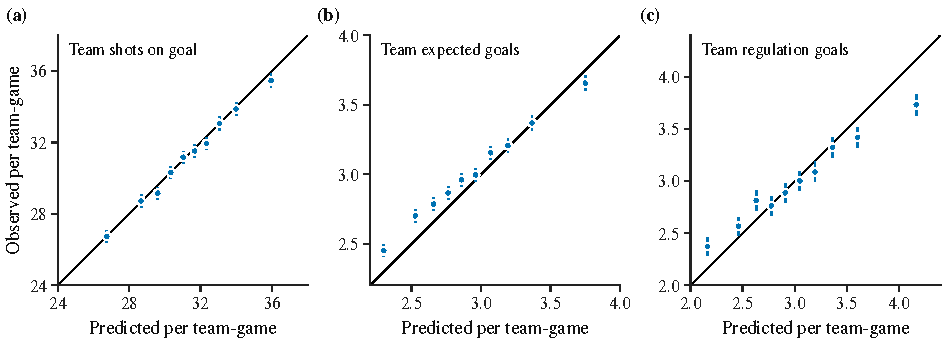
\includegraphics[width=\textwidth]{fig_team_box}
\caption{\neurhlG{} team box-score predictions on the gate window (12,536 to
12,578 team-games): mean outcome by decile of prediction, with 95\% intervals, for
team shots on goal, expected goals and regulation goals, against the identity
line.}
\label{fig:teambox}
\end{figure}

\begin{figure}[t]
\centering
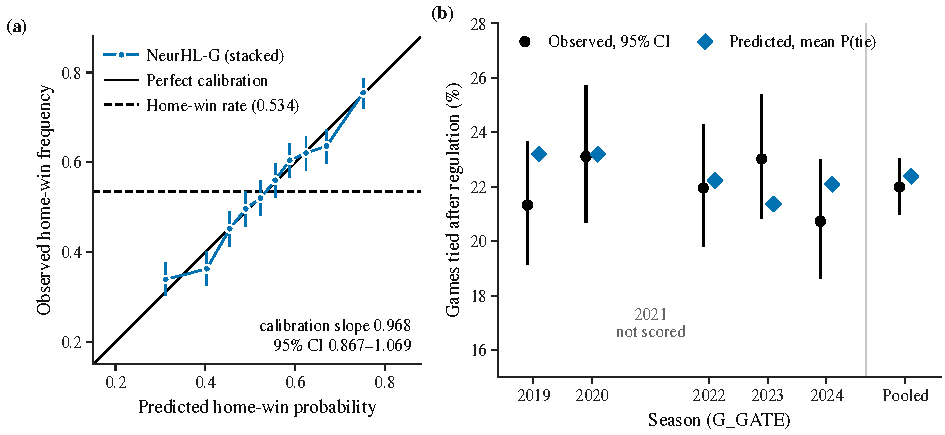
\includegraphics[width=\textwidth]{fig_outcome_calib}
\caption{\neurhlG{} outcome calibration on the gate window. (a) Reliability of
the final home-win probability in equal-count bins, with the calibration slope
and its 95\% interval. (b) Predicted and observed share of games tied after
regulation, by season and pooled; the prediction comes from the hazard
integration, with no tie scalar.}
\label{fig:otcal}
\end{figure}

\paragraph{Reading.}
Two independently built models that both condition on the dressed lineup, one
a small residual network over player histories feeding a four-feature logistic
head, the other a conservation-constrained engine that models every skater's
deployment and every team's scoring process, arrive at nearly the same
win-probability skill. On the iteration window the engine adds nothing beyond
\neurhlH{}, and on the gate window it adds an amount indistinguishable from zero.
We read this as evidence that the binding constraint is the information
available before the game, not the capacity or structure of the model; the
engine's value is that it produces a coherent box score at that same level of
skill.

\subsection{Development only: seasons and player seasons}
\label{sec:res-season}

The season simulator's 80\% intervals cover 0.794 of team-seasons, with a
standings error of 9.61 points (MAE) and a CRPS of 6.93, pooled over the
development and tune seasons. Its interval width was tuned on the same
seasons, so these are development numbers. On the five seasons that both its
record and the Elo baseline's share, the Elo baseline is more accurate: 9.17
against 9.99 points MAE and a CRPS of 6.43 against 7.17, ahead in four of five
seasons ($p = 0.19$). An earlier claim that the season layer beat the house
benchmarks compared different seasons and is withdrawn
(Section~\ref{sec:failures}). For player seasons, the declared 50/50 blend of a
gradient-boosted season model and the summed player-game layer had the lowest
points error over 11 vantages (9.07 points per 82 games, against 9.41 and 9.77
for the two paths alone).

\subsection{Documented nulls}
\label{sec:res-nulls}

Table~\ref{tab:nulls} lists the hypotheses that failed. Two deserve comment.
The first neural game model, a 1.2-million-parameter roster network over
player embeddings from an event language model, finished level with a constant
home-win rate. A regularised logistic regression on the same mean-pooled
embeddings did no better (0.6888 against 0.6898), while two team-form features
alone scored 0.6780, and adding the embeddings to form made it worse. A linear
model cannot be accused of failing to optimise, so the signal was absent from
the representation. The embeddings did learn something: position is linearly
decodable from them with 95\% accuracy, and linear probes recover
$R^2 = 0.54$ of points per 60 minutes and $0.59$ of ice time per game, although
neither was ever a training target. They encode what kind of player someone is, not how good his
team is, and every roster carries a similar mix of roles. The second is the
game-level reattempt of the third plan: four blocks of new information
(absence-based replacement value, goalie quality, schedule density, schedule
strength), each added to \neurhlH{}'s head in a declared order, each made the pooled
log loss worse, so no candidate reached the pre-gate.

\begin{table}[t]
\centering
\small
\caption{Documented null results. Each hypothesis was declared before its test
and failed on the stated evidence.}
\label{tab:nulls}
\begin{tabular}{p{0.44\textwidth}p{0.48\textwidth}}
\toprule
Hypothesis & Result \\
\midrule
A neural game network over event-model player embeddings beats Elo & Five configurations; best 0.6966 against Elo 0.67585 and a constant 0.6898 (tune window) \\
Pooled player embeddings carry team strength & Logistic probe 0.6888, level with the constant; embeddings added to team form make it worse \\
A career encoder can place rookies & Validation error 0.99--1.00 of predicting the mean at every vantage \\
Neural player-rate heads beat a player's own average & Worse on ice time (MAE 0.00934 against 0.00619) and shots; level with a shrunk average on goals \\
The event simulator's rates beat Elo per game & Blend 0.67763 against Elo 0.67668; its pre-gate stopped the confirmation \\
Absences, goalie quality, schedule density or strength improve the game head & Each block adds log loss (+0.00024 to +0.00541) \\
A starter model beats simple heuristics & Season start share wins (log loss 0.66--0.68 against 0.71--0.77) \\
Goals saved above expected predicts next season better than shrunk save percentage & $r = 0.159$ against $0.218$; Steiger $p = 0.007$ in favour of save percentage \\
RAPM transfers to a new team better than team-demeaned raw rates & Indistinguishable (movers $r = 0.387$ against $0.371$, $p = 0.60$) \\
The shot-quality model is calibrated to 0.005 per decile & Best 0.0065 after three declared correction ladders \\
\neurhlG{} adds win-probability information beyond \neurhlH{} & $-0.00049$ (SE 0.00060) on the gate window; the pre-gate failed \\
\bottomrule
\end{tabular}
\end{table}

\section{Failures and corrections}
\label{sec:failures}

The protocol did not prevent mistakes. It made them visible, and it fixed in
advance what each one would cost. This section records the ones that changed
a result or a claim.

\subsection{Leaks that realism gates could not see}

The event simulator passed its preregistered realism gates, per-period event
rates and score effects, with two leaks present. The first was an orientation
flag equal to the team that owned the \emph{next} event, which is the team
component of the prediction target; it agreed with the target's team in every
held-out step. The second was worse. The model conditioned on the on-ice
players at the next event, and because line changes happen at stoppages, a
change in on-ice personnel announces the faceoff that caused it: when the
next event's on-ice set lost one skater, the next event was a faceoff with
probability 0.986 against a base rate of 0.199. About 3,000 of 62,094 held-out
steps were given a near-deterministic answer.

Neither gate could catch either leak, because both scored the model on the
inputs it had been trained with, and a leaked input improves realism along
with everything else. The first leak surfaced only when a downstream consumer
had to supply the flag itself and produced a home scoring rate of 0.39 goals
per 60 minutes against 3.30 for the away side; the second surfaced in the audit
that followed. The fix conditions on the current on-ice set and fixes the
orientation, which lowers the actor head's ceiling honestly: the next actor is
on the ice for 59.6\% of steps, against the 82.7\% the leaked version enjoyed.
All earlier results for the simulator were voided and every seed was
retrained. The lesson generalised into the standing causality audit of
Section~\ref{sec:protocol}: leakage needs either a consumer that must supply
every input itself or a direct test of causality; realism is not evidence of
legitimacy.

\subsection{A measurement drift}

The shot-quality model's calibration gate failed three times, and each failure
was diagnosed on training-side seasons before the next correction was
declared. First, the calibrator had been fitted on cross-validation folds and
applied to a model trained on all the data, which was better calibrated than
the folds, so calibration made it worse (maximum decile deviation 0.0088
against 0.0061 uncalibrated on a development vantage). Second, the recording
change of Section~\ref{sec:data} moved the meaning of a shot location from 2023
on; a calibrator frozen at the end of the previous season is exactly one
season behind a moving target. The declared remedy refits the isotonic map
within the season on trailing out-of-sample shots. Third, per-rink recording
offsets were added as walk-forward covariates. The pooled maximum decile
deviation fell from 0.0222 to 0.0124 and then to between 0.0060 and 0.0074
across the later declared stages, but never reached the 0.005 bar. The failure
is recorded against the transition itself, which no walk-forward method can
see before it happens.

The same drift reached \neurhlG{}. Trained through 2024, it learned the older ratio
of goals to expected goals and reads 2025--26-era expected goals as inputs, so
a dry run on opening night projected 3.36 regulation goals per team-game
against a league level near 3.0. Because the win-probability stack is fitted on
the engine's unscaled outputs and the box-score simulation conditions every
score on the stacked outcome, the win probabilities are unaffected; only the
stat sheet's scoring level is. A declared amendment, committed before any
2026--27 game, scales the stat sheet's goal means by a factor fixed before the
season and updated walk-forward (Section~\ref{sec:live}).

\subsection{Protocol corrections}

\paragraph{A rule changed with the result in view.}
The first plan's fourth amendment required every headline result to be
reported both with and without the anomalous seasons. A later plan replaced
that rule with a simpler one, train but never score 2013 and 2021, and called
the replacement a verbatim carry-over. It was not: the replacement was written
after tune-window results were visible, and the commit that introduced it also
recorded \neurhlH{}'s tune-window pass ($p = 0.0075$). Between the committed tune
failure ($p = 0.120$) and that pass, three defensible things had changed on the
same window: the scored seasons, two corrections to Layer~1, and the scoring
rule. Together they were decisions taken with the result in view. A later
amendment reclassified the tune-window result as exploratory, required it to
be reported under every scored set ($p$ from 0.0075 to 0.019), and declared the
one-shot confirmation reported in Section~\ref{sec:res-h}.

\paragraph{A comparison across different seasons.}
An early summary stated that the season layer beat both house benchmarks. The
benchmark figure came from 2018--2026 and the \neurhl{} figure from 2011--2017.
On matched seasons the Elo baseline is better (Section~\ref{sec:res-season});
the claim is withdrawn.

\paragraph{Reliability is not validity.}
The first RAPM gate required split-half reliability above that of raw on-ice
shot share, and RAPM failed it (offence 0.656 against 0.789). The gate was
wrong: raw on-ice rates are more repeatable because they are contaminated, as
a player keeps the same linemates, zone starts and competition in both halves,
and RAPM removes exactly those terms. Ranking rating systems by reliability
rewards confounding. The gate was retired and replaced by predictive transfer
to a new team, on which RAPM tied a one-line team-demeaned baseline.

\paragraph{Gates implemented short of their declaration.}
While writing this paper we found that the script implementing \neurhlG{}'s gates
had omitted three declared components: the randomised-PIT coverage criterion
of the calibration gate, the comparison against the summed player-game layer,
and CRPS. The calibration gate had been judged on its slope and overtime share
alone and recorded as a pass. Computed afterwards from the same saved
predictions, with nothing refitted, the team-box-score comparisons pass but the
coverage for team shots is 0.860 against a nominal 0.80 and a tolerance of 0.03,
so the calibration gate fails as declared. The correction was appended to the
plan as a dated amendment. It changes no decision, because the pre-gate had
already failed on its \neurhlH{} condition, but it changes a public claim, and
Table~\ref{tab:gates} reports the corrected record.

\section{The 2026--27 prospective test}
\label{sec:live}

Every season through 2026 has now been used at game level by some part of
\neurhl{}, so the 2026--27 season, which begins on 29 September 2026, is the
only data on which all the models can be tested cleanly. Two sets of
predictions are scored.

\paragraph{Frozen preseason predictions.}
On 25 September 2026, four days before opening night, \neurhl{} 1.0 committed
static predictions with their SHA-256 hashes: a home-win probability for each
of the 1,344 regular-season games, team points with 80\% intervals and
playoff probabilities from 20,000 simulated seasons, and goals, assists and
points for 711 skaters. The scoring plan fixes the statistics in advance (per-game
log loss against the preseason Elo reference; standings error and interval
coverage against a house benchmark; skater points error for the shipped blend
and its two components), states the expected outcomes, including that Elo is
expected to win the per-game comparison because the season engine behind these
probabilities scored worse than Elo on the tune window, and allows one
inference only, after the last regular-season game. After the NHL roster
deadline on 28 September a dated update re-runs the same frozen models on the
final rosters, with availability entries such as a goaltender suspended by his
club removed. It is hashed and scored beside the originals, which remain
primary.

\paragraph{Game-day forecasts.}
\neurhlG{} is live as an exploratory model and \neurhlH{} as the primary win-probability
model. The live engine is the candidate trained through 2024. Its stack,
fitted on out-of-sample predictions for 14,940 games of 2011--2024, puts
coefficients of 0.21, 0.29 and 0.58 on the Elo, \neurhlG{} and \neurhlH{} logits
(0.63 and 0.46 on Elo and \neurhlG{} when \neurhlH{} is unavailable). Each game day produces a morning forecast at about 11:00 Eastern time
with projected lineups and a pregame forecast 45 to 75 minutes before the
scheduled start with the latest lineups and starting goalies. Each forecast
records where its lineup came from: the league's own game data, confirmed
lines, projected lines, or a fallback built from the team's last dressed roster
minus unavailable players. A forecast counts only if the commit that adds it is
on the public repository's main branch before the scheduled start, checked
against the remote and dated independently by a hosted continuous-integration
run. A game without a valid forecast is counted as missed for every model, so
that missing data cannot favour one of them, and nothing is backfilled. The
pregame forecast is primary and the morning forecast secondary. In-season Elo
and \neurhlH{}, fed the same lineups, are scored on the same games, and the frozen
1.0 probabilities are reported descriptively. Inference is made once, after
the last regular-season game, with a bootstrap over weeks of play. With about
1,300 games the standard error of a paired difference is about 0.0024, so only
gaps of about 0.007 or more are likely to be resolved within the season.

\paragraph{The stat sheet's scoring level.}
Because of the recording drift, \neurhlG{}'s stat sheet is scaled by a declared
factor $m$ that multiplies regulation goal means (and so assists) and leaves
win probabilities unchanged. Before the season, $m_0 = L / M$, where $L$ is the
previous season's league regulation goals per team-game computed from the era
inputs the model already receives and $M$ is the engine's own mean projected
regulation goals over every game in the first 14 days, computed from roster
fallback lineups. In season,
\begin{equation}
m = \frac{A + kL}{P + kM}, \qquad k = 300 \text{ team-games},
\end{equation}
where $A$ and $P$ are the actual and unscaled predicted regulation goals over
completed 2026--27 games that have a primary forecast, so the factor moves
from $m_0$ toward the observed ratio as games accumulate and a forecast only
ever uses games already finished. On rosters from the day before the deadline
the factor was 0.922; it is fixed on the final rosters before the first game.

\paragraph{What the season can show.}
A single season cannot confirm effects of the size reported in
Section~\ref{sec:results}. Its purpose is prospective accountability: every
forecast is public before the event it forecasts, the scoring rules are fixed,
and the results will be published whatever they show. We will report them in
a revision of this paper after the regular season ends on 10 April 2027.

\section{Discussion}
\label{sec:discussion}

\paragraph{Information, not capacity.}
The same pattern recurs at every level of the project. A 1.2-million-parameter
roster network over event embeddings finished level with a constant; a linear
probe on the same embeddings did no better; two team-form features beat both.
Tree ensembles on engineered game features did not beat Elo. A small residual
network that reads the dressed lineup did beat Elo, confirmed on eight seasons,
and a far more structured engine that models every skater's deployment and
every team's scoring process reached the same skill and no more. What moved
the result was information that Elo does not use, namely who is dressed and
what those players have done, rather than any particular architecture. The
exploratory split in Section~\ref{sec:res-h} points the same way: \neurhlH{}'s
gain is near zero when neither team is missing regulars and largest when one
team is missing far more than the other. We
expect further gains to come from new information available before a game,
such as tracking data, line deployment and injury reports with dates, rather
than from larger models of the information already used.

\paragraph{What preregistration changed.}
The protocol altered this project's conclusions in concrete ways. It turned an
apparently significant tune-window result into an exploratory one and forced
a one-shot confirmation, which then passed. It withdrew a season-level claim
that rested on mismatched seasons. It retired a gate that would have selected
the more confounded rating system. It kept two confirmatory windows unspent
when pre-gates failed, including \neurhlG{}'s sealed seasons, which remain
available to a better candidate. It recorded, before the gate ran, that \neurhlG{}
was expected to fail its pre-gate, so the failure cannot be explained away
afterwards. None of these outcomes flatter the models; all of them make the
confirmed results more credible.

\paragraph{Audits over gates.}
Both leaks in the event simulator passed every realism gate, and the gate
implementation errors in Section~\ref{sec:failures} passed our own review
until the results were written up in full. Gates check what a model does with
its inputs; they do not check the inputs or the checkers. The two mechanisms
that caught these problems were a consumer that had to supply every input
itself and a direct causality test, and the act of restating every gate
against its declaration for publication.

\paragraph{Limitations.}
The \neurhlG{} gate seasons had been scored at game level by \neurhlH{} before \neurhlG{}
existed, so the gate result is evidence, not confirmation. The evaluation
covers one league and seasons 2008--2026, whose most recent years include a
change in how shots are recorded. Market data were excluded by design and no
historical odds exist in the repository, so we cannot say how close the
models come to the market. \neurhlH{}'s head selects its regularisation on training
loss, a weakness kept for the confirmation. Several claims about the season
layer and player seasons rest on development evidence only. Neural training
is not bit-reproducible on the hardware used, which we address by hashing
checkpoints and reporting CPU inference, but a retrained model will differ
slightly from the published one. Finally, in-season expected goals for
2026--27 depend on a third-party shot file being published on time.

\paragraph{Future work.}
The live season will provide the first clean test of \neurhlG{} and a second,
prospective test of \neurhlH{}. The sealed seasons 2025--2026 remain available for a
single confirmatory test of a future \neurhlG{} candidate under a new plan, which
could spend it with one declared change after the failed pre-gate, as the
current plan allows, or with a new model that brings new information.
Candidate information sources include player tracking data, available from
2022 but absent from most of the history, deployment models that predict line
combinations, and injury and scratch reports with reliable timestamps.

\section{Conclusion}
\label{sec:conclusion}

Under a protocol that fixed windows, gates and consequences in advance, a
neural player-level model conditioned on the dressed lineup beat a tuned Elo
system on eight held-out NHL seasons by 0.0048 nats per game, with a
confidence interval that excludes zero comfortably and a gain that comes from
resolution. A chained player-game model beat each skater's own history on all
four of its targets. A single-game simulation engine reached the same
win-probability skill as the confirmed model while producing a coherent box
score, but did not exceed it, so its sealed test was kept for a future
version. Most of what we tried did not work, and the record of those failures,
including our own errors, is part of the result. All forecasts for the
2026--27 season are public before their games and will be scored once, at the
end of the season.

\paragraph{Code and data availability.}
Code, preregistrations, search ledgers, committed predictions and the
acceptance tests that re-derive them are at
\url{https://github.com/ph05/neurhl}. Raw play-by-play, shift and tensor files
are not redistributed; the repository's fetchers rebuild them from the public
sources named in Section~\ref{sec:data}.


\bibliographystyle{plainnat}
\bibliography{refs}

\clearpage
\appendix
\section{Preregistration timeline}
\label{app:timeline}

Table~\ref{tab:timeline} lists the commits that fixed each plan, amendment,
candidate and freeze, with their commit times (Eastern time). The repository
became public on 26 September 2026; earlier times are as recorded in its
history, and later commits are also dated by their push to the public branch.
Commit identifiers quoted inside the plan documents predate publication and are
mapped to the public history in \texttt{neurhl/configs/commit\_map.csv}.

\begin{table}[H]
\centering
\small
\caption{Commit times of the preregistration record, 2026.}
\label{tab:timeline}
\begin{tabular}{llp{0.58\textwidth}}
\toprule
Date & Time & Commit \\
\midrule
20 Aug & 10:38 & First plan locked with tune-window baselines, before any gate ran \\
20--21 Aug & & Amendments 1--4 (team form; significance test S1; shot-based form; lockout season), each before its run \\
21 Aug & 13:32 & Second plan (event simulator, season layer), before any of its numbers \\
21 Aug & 23:17 & Amendment 8: two simulator leaks recorded; earlier simulator results voided \\
24 Aug & 14:48 & Third plan (player, goalie and game layers) and the rink ladder \\
25 Sep & 14:46 & First plan, Amendment 5: record correction and the frozen one-shot confirmation of \neurhlH{} \\
25 Sep & 15:06 & Live plan: 2026--27 predictions frozen with hashes \\
27 Sep & 12:33 & Fourth plan (\neurhlG{}), before any \neurhlG{} number \\
27 Sep & 16:07 & \neurhlG{} candidate declared, before any gate number \\
27 Sep & 17:24 & \neurhlG{} freeze: gate results, pre-gate failed, seal unspent \\
27 Sep & 17:55 & Stat-sheet goal-level amendment, before any 2026--27 game \\
27 Sep & 22:56 & Gate record correction (Section~\ref{sec:failures}) \\
\bottomrule
\end{tabular}
\end{table}

\section{\neurhlG{} configuration}
\label{app:config}

\begin{table}[H]
\centering
\small
\caption{\neurhlG{} candidate g1. The configuration file's SHA-256 begins
\texttt{587746c6}; the master tensor's begins \texttt{325390c3}.}
\label{tab:config}
\begin{tabular}{lp{0.58\textwidth}}
\toprule
Setting & Value \\
\midrule
Skater, goalie, team, context features & 114, 23, 57, 10 per game side \\
State decays (per game) & 0.98, 0.95, 0.85, 0.60 \\
Encoders & skater 116--128--64; team 57--64--32; goalie 23--32--16; context 10--32--16 \\
Heads (zero-initialised output) & skater 112--64--12; team 112--64--6; goalie 32--32--1 \\
Activation, normalisation, dropout & GELU, layer norm, 0.2 \\
Parameters & 48,810 \\
Hazard table & 7 leads $\times$ 5 phases, initialised from the event simulator \\
Integration & goal differential $-8$ to 8; 30 steps of 2 minutes; 5 Gauss--Hermite nodes \\
Phase 1 & 10 epochs, AdamW, learning rate $2\times10^{-3}$, weight decay 0.01, outcome weight 0.3 \\
Phase 2 & 4 epochs, learning rate $3\times10^{-4}$, outcome weight 1, L2-SP $10^{-3}$ \\
Batch, schedule, gradient clip & 256 games, one-cycle, 5.0 \\
Training seasons for snapshot $T$ & 2009 to $T-1$ \\
Ensemble & 5 seeds \\
Final probability & logistic stack over Elo, \neurhlG{} and \neurhlH{} logits; subset by leave-one-season-out cross-validation \\
Stat sheet & 10,000 draws per game; team shots negative binomial, $r = 40$ \\
\bottomrule
\end{tabular}
\end{table}

\section{Definitions}
\label{app:defs}

\paragraph{Log loss and paired differences.}
For a home-win indicator $y_g$ and forecast $p_g$, the per-game log loss is
$\ell_g = -y_g \log p_g - (1 - y_g)\log(1 - p_g)$. Model comparisons use
$\bar d = n^{-1}\sum_g (\ell^{A}_g - \ell^{B}_g)$ over the same $n$ games.

\paragraph{Murphy decomposition.}
With forecasts grouped into bins $k$ of size $n_k$, mean forecast $\bar p_k$ and
observed frequency $\bar y_k$, and overall frequency $\bar y$, the Brier score
is reliability minus resolution plus uncertainty:
$n^{-1}\sum_k n_k(\bar p_k - \bar y_k)^2 - n^{-1}\sum_k n_k(\bar y_k - \bar y)^2
+ \bar y(1 - \bar y)$.

\paragraph{Randomised PIT.}
For a count $y$ with predictive distribution function $F$, the randomised
probability integral transform is $u = F(y-1) + v\,[F(y) - F(y-1)]$ with
$v \sim \mathrm{U}(0, 1)$, as reviewed by \citet{czado2009predictive}. Under a calibrated forecast
$u$ is uniform, so the share of $u$ in $[0.1, 0.9]$ estimates the coverage of a
central 80\% interval without the over-coverage of discrete intervals.

\paragraph{Wild cluster bootstrap.}
With $S$ season-level mean differences $\bar d_s$, the statistic is recomputed
under every one of the $2^S$ sign patterns $\epsilon \in \{-1, 1\}^S$ applied to
the season means, which gives an exact sign-flip $p$-value;
with eight seasons the smallest attainable two-sided value is $2/256 = 0.0078$.

\paragraph{log5.}
For a team rate $a$ and an opponent's allowed rate $b$ in a league with mean
rate $L$, $\mathrm{log5}(a, b) = ab/L$.

\section{Reproducibility}
\label{app:repro}

The repository needs Python 3.12 and \texttt{uv}; there is no environment to
install. Four acceptance batteries re-assert every recorded gate decision
against its declared rule, re-derive committed predictions on CPU within
$10^{-6}$, check ledger caps and window guards, and confirm that each one-shot
window was spent at most once. At the time of writing they pass 25 of 25, 40 of
40, 25 of 25 and 10 of 10 checks. The frozen 2026--27 files and their SHA-256
prefixes are the game probabilities (\texttt{85565efd}), the team projections
(\texttt{4c60f50f}), the skater projections (\texttt{cc4cc26d}) and the house
benchmark (\texttt{a4a693f4}). Per-game predictions for the \neurhlH{} confirmation
and for the \neurhlG{} iteration and gate windows are committed under
\texttt{neurhl/output/preds/}, and every figure in this paper is regenerated
from committed files by \texttt{paper/figures/make\_figures.py}.


\end{document}
